\section{System Model}
%----------------------------------------------------------------------------------------%
\subsection{Network Model}
We consider an edge computing system with $K$ Access Points (APs) and $M$ edge servers, which are connected in a network as illustrated in Fig.\ref{fig:system}.
The sets of APs and edge servers are denoted as $\apSet \define \set{1,\dots,K}$ and $\esSet \define \set{1,\dots,M}$, respectively.
Without loss of generality, it is assumed that there are $J$ types of computation jobs supported in this system, which are denoted via the set $\mathcal{J} \define \set{1,\dots,J}$.
Each AP collects the computation jobs from the mobile users within its coverage, and makes decision on the processing edge servers for each job type from the set $\esSet$.
It is assumed that the $k$-th AP only dispatches the computation jobs to the feasible edge servers, e.g. the edge servers within a certain number of hops.
Let $\esSet_{k} \subseteq \esSet$ be the set of edge servers, which can compute the jobs from the $k$-th AP and $\apSet_{m}$ be the set of APs, which may upload jobs to the $m$-th edge server.
We refer to $\esSet_{k}$ as the \emph{candidate server set} of the $k$-th AP, and $\apSet_{m}$ as the \emph{candidate AP set} of the $m$-th edge server ($\forall k\in\apSet, m\in\esSet$).
% As illustrated in Fig.\ref{fig:conflict},
Different APs may have different candidate servers according to their locations in the network.
For example, it is possible that $\esSet_{k} \neq \esSet_{k'}$ and $\esSet_{k} \cap \esSet_{k'} \neq \emptyset$ when $k \neq k' \in \apSet$.
\accept{
    In this edge computing network, each AP decentralized makes job dispatching decision faciliated by inforamtion sharing from other APs and edge servers.
}
Specifically, each AP and edge server periodically broadcast their state information (e.g. edge server dispatching choice for each job type, list of jobs being uploaded from APs to edge servers, computing queue length and etc.), and one AP updates its strategy on job dispatching when receiving the broadcast state information.
In this paper, we shall optimize the job dispatching strategy at APs with part of the broadcast information and random broadcast latency.

\begin{figure}[ht]
    \centering
    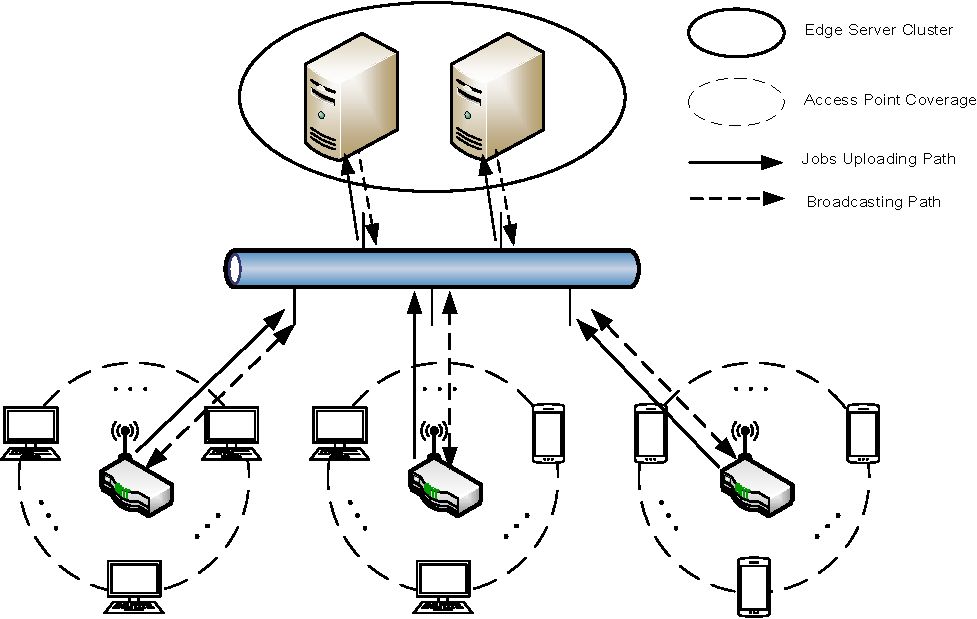
\includegraphics[width=0.80\textwidth]{system-model.pdf}
    \caption{The Illustration of MEC System Model}
    \label{fig:system}
\end{figure}

%NOTE: [job space support and arrival process]
The time axis is organized by time slots.
The job arrivals in each time slot on each AP are modelled via independent Bernoulli distributions.
Specifically, the arrivals of the $j$-th job type at the $k$-th AP in different time slots are independent and identically distributed (i.i.d) Bernoulli random variables, and the arrival probability is denoted as $\lambda_{k,j}$ ($\forall k\in\apSet, j\in\jSpace$).
Let $A_{k,j}(t) \in \set{0,1}$ represents the event of job arrival, where $A_{k,j}(t)=1$ means one job of the $j$-th job type arrives on the $k$-th at the $t$-th time slot, and $A_{k,j}(t)=0$ means other wise.
Hence,
\begin{align}
    \Pr\{ A_{k,j}(t) = 1 \} = \lambda_{k,j}, \forall t,k\in\apSet,j\in\jSpace
\end{align}

%NOTE: [uploading process]
Each AP then immediately dispatches each type of received jobs to one edge server.
Different types of jobs may have different distributions on the input data size.
Moreover, due to the random traffic in the network, the job uploading from one AP to one edge server consumes a random number of time slots.
It's assumed that the distributions of uploading time are independent between any two uploading jobs.
Hence, we denote $\mathcal{U}_{k,m,j}$ as the uploading time for the $j$-th job type uploading from the $k$-th AP to the $m$-th edge server following some distribution with support $\set{1, \dots, \Xi}$, where $\Xi$ denotes the maximum uploading time ($\forall k\in\apSet, m\in\esSet, j\in\jSpace$).
In practice, the distribution of uploading latency may not be known to the APs or edge servers in advance.

%NOTE: [processing process]
There are $J$ virtual machines (VMs) running parallel on each edge server for the computation of $J$ job types, respectively.
For each job type, the uploaded jobs are computed in a First-Come-First-Serve (FCFS) manner.
Hence, a processing queue with maximum $L_{max}$ jobs is established for each VM.
The arrival jobs will be discarded when the processing queue is full.
Furthermore, we adopt the \emph{unrelated machines assumption} in \cite{tan-online} for job processing on edge servers.
Specifically, it is assumed that the computation time of different job types on different edge servers follows the memory-less Geometric distribution (with the unit of time slot) with different expectations.
Let $C_{m,j} \sim \mathbb{G}(1/c_{m,j})$ be the computation time distribution of the $j$-th job type on the $m$-th edge server, where $c_{m,j}$ is the expectation.
Hence, the probability mass function (PMF) of $C_{m,j}$ is given by:
\begin{align}
    f_{m,j}(k) \define (1-\frac{1}{c_{m,j}})^{k-1} \frac{1}{c_{m,j}}.
\end{align}
%----------------------------------------------------------------------------------------%

\subsection{Periodic Broadcast of State Information}

\begin{figure}[ht]
    \centering
    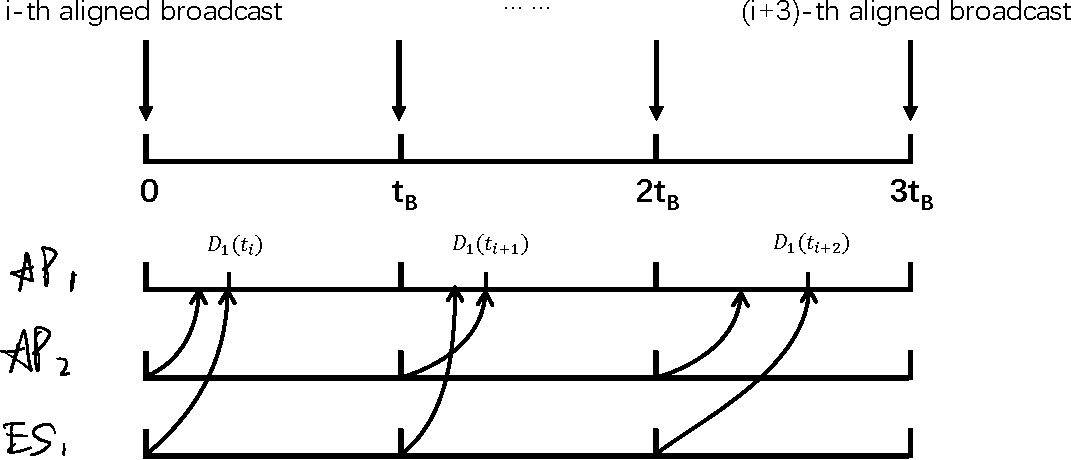
\includegraphics[width=0.80\textwidth]{brd-timeline.pdf}
    \caption{The timeline illustration of LSI broadcast with 2 APs and 1 edge server.}
    \label{fig:brd-timeline}
\end{figure}

%NOTE: Periodic Broadcast is Indispensable
In order to facilitate cooperative dispatching for the APs, it is assumed that all the APs and edge servers will broadcast their \emph{local state information} (LSI) every $t_B$ time slots as depicted in Fig.\ref{fig:brd-timeline}.
We shall refer to every $t_B$ time slots as a broadcast interval.
At the beginning of each broadcast interval (say the $t$-th broadcast interval), the LSI of each AP and edge server is defined below, respectively.

%NOTE: State and Broadcast Information for AP
\begin{definition}[Local State Information for AP]
    One AP shall maintain LSI about the number of jobs in uploading, and the dispatching choice on edge server for each job type.
    Specifically, at the $n$-th time slot in the $t$-th interval, the number of the $j$-th type job being uploaded to the $m$-th edge server $\xi$ time slots ago from $k$-th AP is denoted as $R^{(k)}_{m,j,\xi}({t,n})$ ($\forall k\in\apSet, m\in\esSet, j\in\jSpace, \xi\in(0,\Xi]$);
    the dispatching choice of the $k$-th AP for processing of the $j$-th job type is denoted as $\omega_{k,j}(t,n) \in \esSet_{k}$.
    Hence, the LSI of the $k$-th AP at the $t$-th broadcast is given as follows.
    \begin{align}
        \mathcal{R}_{k}({t}) \define \set{\vec{R}^{(k)}_{m,j}({t}), \set{\omega_{k,j}(t)|\forall j\in\jSpace} | \forall m\in\esSet, j\in\jSpace},
    \end{align}
    where $\vec{R}^{(k)}_{m,j} \define ( R^{(k)}_{m,j,0},\dots,R^{(k)}_{m,j,\Xi} )$ denotes the vector of random variables for convenience; and we have index $t$ short for $(t, 0)$, i.e. the beginning time slot of the $t$-th broadcast interval.
\end{definition}

%NOTE: State and Broadcast Information for ES
\begin{definition}[Local State Information for Edge Servers]
    One edge server shall maintain LSI about the computing queue status for each VM.
    Specifically, at the $n$ time slot in the $t$-th interval, the $m$-th edge server have $Q_{m,j}({t,n})$ denote the pending number of the $j$-th type job ($\forall m\in\esSet, j\in\jSpace$).
    Hence, the LSI of the $m$-th edge server at the $t$-th broadcast is defined as follows.
    \begin{align}
        \mathcal{Q}_{m}({t}) \define \set{Q_{m,j}({t}) | \forall j\in\jSpace},
    \end{align}
    where we have index $t$ short for $(t, 0)$, i.e. the beginning time slot of the $t$-th broadcast interval.
\end{definition}

And we refer to the \emph{global state information} (GSI) as the composition of all the broadcast information from all APs and edge servers in one broadcast of which the definition is given as follows.
\begin{definition}[Global State Information]
    \begin{align}
        \Obsv^{\dagger}(t) \define
            \Brace{
                \mathcal{R}_{k}({t}), \mathcal{Q}_{m}({t}) | \forall k\in\apSet, m\in\esSet
            },
    \end{align}
    which is composed of all the broadcast information from all APs and edge servers at the $t$-th broadcast.
\end{definition}

In \comments{an extensive edge computing network residing in MAN}, it may not be feasible for each AP to collect the LSI from all other APs and edge servers.
Moreover, the transmission latency of LSI in \comments{such extensive edge computing network} is not negligible.
It is assumed that the $k$-th AP is able to collect the OSI $D_{k}(t)$ time slots later after the broadcast of the $t$-th interval, where $D_{k}(t)$ is a random variable follows some distribution.
As a high frequency broadcast design would always result into \emph{broadcast storm} and block the normal network traffic \needref{broadcast-storm article}, we introduce a slow enough broadcast interval selection in the system.
The broadcast interval is always larger than the maximum \brdelay, i.e. $t_B > \hat{D}_k$ ($\forall k\in\apSet$), where $\hat{D}_k$ is the upper bound for $D_{k}({t})$.
Hence, $D_{k}(t)$ follows some distribution with support $\set{1,\dots,t_B}$, i.e. the broadcast interval $t_B$ is set that the $k$-th AP ($\forall k\in\apSet$) could receive the complete OSI before the start of next broadcast interval.

\fixit{
    observed information definition should be put into solution part.

    %NOTE: Conflict of AP set and partial information definition
    In \comments{an extensive edge computing network residing in MAN}, it may not be feasible for each AP to collect the LSI from all other APs and edge servers.
    Hence, we first define the \emph{conflict AP set} as follows.
    \begin{align}
        \ccSet_{k} \define \bigcup_{m\in\esSet_{k}} \apSet_{m}
        % \ccSet_{k} \define \set{\forall k' \neq k\in\apSet|\esSet_{k'} \cap \esSet_{k} \neq \emptyset}
    \end{align}
    The \emph{conflict AP set} indicates the subset of APs whose LSI could affect the decision making for the $k$-th AP.
    It is assumed that each AP can only collect the LSI from the APs in its \emph{conflict AP set} and edge servers from its \emph{candidate server set}.

    \begin{definition}[Global State Information]
        Hence, we can define the \emph{observed state information} (OSI) of the $k$-th AP as follows.
        \begin{align}
            \Obsv_{k} &= \set{\mathcal{R}_{k'} | \forall k'\in\ccSet_{k}}
                            \cup \set{\mathcal{Q}_{m} | \forall m\in\esSet_{k}},
        \end{align}
    \end{definition}

    One AP will update its dispatching decision after the reception of its OSI.
    Specifically, let $\omega'_{k,j}(t)$ be the new computing edge server for the $t$-the broadcast interval, the $k$-th AP should determine th new policy $\omega'_{k,j}(t)$ in the $D_{k}(t)$ time slot of the $t$-th broadcast interval.

    We denote the individual dispatching policy of the $k$-th AP ($\forall k\in\apSet$) based on its OSI $\Obsv_{k}({t})$ ($t \in\domP$) as follows.
    \begin{align}
        &\Omega_{k}(\Obsv_{k}(t)) \define \set{\omega'_{k,j}(t)|\forall m\in\esSet, j\in\jSpace}.
        \label{def_action}
    \end{align}
    And we note that the $k$-th AP would always adopt two phases polices in the $t$-th interval, i.e. $\Omega_{k}(\Obsv_{k}({t-1}))$ with $\omega_{k,j}(t)$ before receiving $\Obsv_{k}(t)$ and $\Omega_{k}(\Obsv_{k}(t))$ with $\omega'_{k,j}(t)$ afterwards.
    % The two phases policy of APs in one together determine the transition of $\Obsv({t+1})$ in the next interval.
}

However, the randomness of \brdelay~implies that one AP could not know other APs' \brdelay~in the same interval.
Thus, APs are unable to evaluate the impact introduced by others' policy on the next broadcast information and fail to establish exact cooperation.
An naive way to solve this problem is to force all APs update their policy only at the end of the interval, which introduces a inevitable lagging for a whole broadcast interval.

In the following problem formulation section, we will show that we could come up with better dispatching decision update solution which is aware of the \brdelay, and improve APs' dispatching decisions in an iterative way.
Furthermore, with the help of algorithm design we could prove that our improved policy is with analytical performance bound under MDP framework.


\delete{v6.1}{
    Due to the randomness of the network traffic, the \brdelay~shall be random based on the uncertainty of the arrival latency of each part of information from \emph{candidate server set} of edge servers and \emph{conflict AP set} of APs.
}

\delete{v6.2}{
    \begin{figure}[htp]
        \centering
        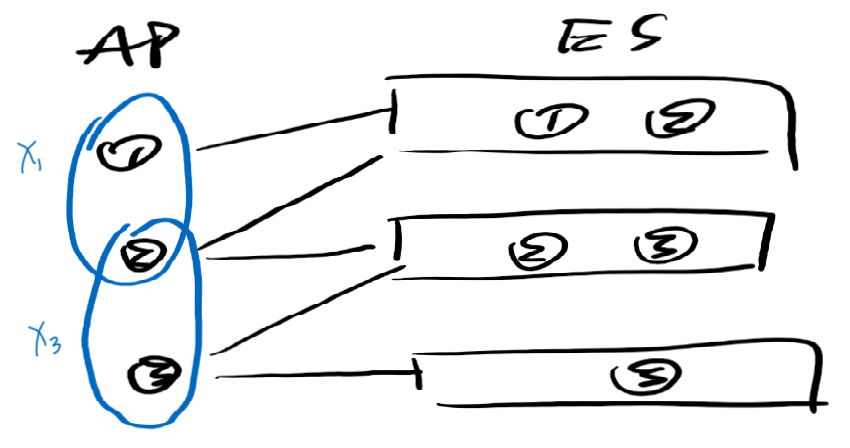
\includegraphics[width=0.80\textwidth]{images/draft-conflict.png}
        \caption{The Example Illustration of Conflict Set and Partial Broadcast Information}
        \label{fig:conflict}
    \end{figure}

    One simple example is given as follows.
    \begin{example}
        As depicted in \ref{fig:conflict}, there are 3 APs and 3 edge servers in the system.
        The \emph{candidate set} for each AP is denoted as: $\esSet_{1}=\set{1}, \esSet_{2}=\set{1,2}, \esSet_{3}=\set{2,3}$, respectively.
        The \emph{conflict set} for each AP is denoted as: $\ccSet_{1}=\set{1,2}, \ccSet_{2}=\set{1,2,3}, \ccSet_{3}=\set{2,3}$.
        And the partial information required for each AP is denoted as follows.
        \begin{align*}
            \Obsv_{1} &= \set{ \mathcal{R}_{2} } \cup \set{ \mathcal{Q}_{1} }
            \\
            \Obsv_{3} &= \set{ \mathcal{R}_{2} } \cup \set{ \mathcal{Q}_{2}, \mathcal{Q}_{3} }
        \end{align*}
        % And we note that
    \end{example}
}
%----------------------------------------------------------------------------------------%